\documentclass[12pt,titlepage,ngerman]{article}

\usepackage[ngerman]{babel}
\usepackage[utf8]{inputenc}
\usepackage{color}
\usepackage[a4paper,lmargin={2,54cm},rmargin={2,54cm},tmargin={2.54cm},bmargin = {2.54cm}]{geometry}
\usepackage{enumitem}
\usepackage{amssymb}
\usepackage{amsthm}
\usepackage{graphicx}
\usepackage{acronym}
\usepackage[backend=bibtex8,style=alphabetic]{biblatex}
\addbibresource{Studienarbeit.bib}
\usepackage{setspace}

\begin{document}
\begin{titlepage}
	\begin{figure}
		\centering
		
\includegraphics[width=9cm]{Bilder/DHBW_MA_Logo.jpg}
	\end{figure}%
	\title{Erfassung biometrischer Daten mithilfe von Smartphones}	
	\date{28.11.2017 - 28.05.2018}
	\author{Torben Brenner und Lukas Seemann}
	\maketitle
\end{titlepage}
\singlespacing
\addcontentsline{toc}{section}{Inhaltsverzeichnis}
\pagenumbering{Roman}
\tableofcontents
\newpage
\section*{Abkürzungsverzeichnis}
\addcontentsline{toc}{section}{Abkürzungsverzeichnis}
\begin{acronym}[*********]
	\acro{TTT}{Test}
\end{acronym}
\newpage
\addcontentsline{toc}{section}{Abbildungsverzeichnis}
\listoffigures
\newpage

\addcontentsline{toc}{section}{Tabellenverzeichnis}
\listoftables
\newpage

\pagenumbering{arabic}
\onehalfspacing
\section{Einleitung}
Das ist unsere Studienarbeit. \footcite[Vgl.][S. 9000]{Test123}

\begin{figure}[h]
	\centering
	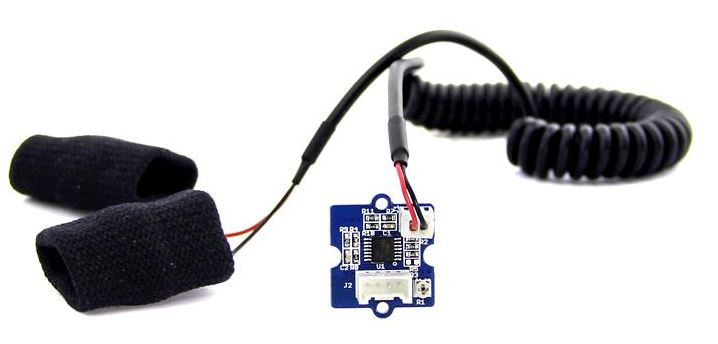
\includegraphics[width=11cm]{Bilder/sensor.jpg}
	\caption{Das ist ein cooler GSR Sensor}
\end{figure}%
\newpage
\section{Theoretische Grundlagen}
\newpage
\section{Hauptteil}
\subsection{Teil 1}
\subsection{Teil 2}
\subsection{Teil 3}
\newpage
\section{Schluss}

\newpage
\addcontentsline{toc}{section}{Literaturverzeichnis}
\printbibliography
\newpage

\section*{Anhänge}
\addcontentsline{toc}{section}{Anhänge}


\end{document}